\documentclass[12pt, titlepage]{report}
\usepackage{consumer_resource_final}
\graphicspath{{./figures/}}

\begin{document}
	\section{Defining the model}
	We want to look at equilibria of a system of $N_R$ resources and $N_S$ species whose evolution is given by:
	\begin{empheq}[left = \empheqlbrace]{align}
	 \dot{R_\alpha} &= \theta_\alpha - \mu_\alpha R_\alpha - \sum_j \gamma_{j \alpha}R_\alpha S_j + \sum_j \alpha_{\alpha j} S_j \\
	 \dot{S_i} &= \sum_\beta \sigma_{i\beta} \gamma_{i \beta } S_i R_\beta - d_i S_i
	\end{empheq}
	Note our specific convention (it is quite important to keep it because stuff can get complicated really quickly) : we use greek indices for resources and latin indices for species. Also we write the species dissipation rate as $d_i$ instead of $\delta_{i}$ to avoid confusion with the Kronecker delta which will be used later. We also write the constant feeding rate of the resource $\theta_\alpha$ instead of $\lambda_\alpha$ to avoid mixing it with eigenvalues of matrices, which we will usually write as $\lambda$.

	In general, the Jacobian matrix $J(R,S)$ of the model is given by:
	\begin{equation}
		J(R,S) = \begin{pmatrix} -(\mu+\gamma^T S)_{d} & -R_d \gamma^T + \alpha \\ S_d \sigma \otimes \gamma & ( (\sigma \otimes \gamma) R - \delta)_d \\ \end{pmatrix}
	\end{equation}
	where $\otimes$ stands for the Hadamard product (element by element).
	The notation $\alpha_d$ is equivalent to $\diag{\alpha}$.
		\subsection{Equilibrium}
	Throughout this paper we will be interested in equilibria of this system, which will be denoted with a star.
	By definition, equilibria solve :
	\begin{empheq}[left = \empheqlbrace]{align}
   	 0 &= \theta_\alpha - \mu_\alpha R_\alpha - \sum_j \gamma_{j \alpha}R_\alpha S_j + \sum_j \alpha_{\alpha j} S_j \label{eq : equilibrium condition 1} \\
   	 0 &= \sum_\beta \sigma_{i\beta} \gamma_{i \beta } S_i R_\beta - d_i S_i \label{eq : equilibrium condition 2}
	\end{empheq}

	 More precisely, we will mostly work with positive valued equilibria \ie $R^*_\alpha > 0$ $\forall \alpha$ and $S^*_i > 0$ $\forall i$. At such a positive-valued equilibrium, the jacobian matrix is given by :
	\begin{equation}
		J^* =
		\begin{pmatrix}
		-D & \Gamma \\
		\beta & Z
		\end{pmatrix}
	\end{equation}

	with
	\begin{itemize}
		\item $D = \left(\mu+\gamma^T S^*\right)_d$, i.e. $D$ is a diagonal $N_R \times N_R$ matrix with strictly positive elements.
		\item $\Gamma = \alpha - R^*_d \gamma^T $ is a $N_R \times N_S$ matrix whose entries do not have a well defined sign.
		\item $\beta = S^*_d \sigma \otimes \gamma $ is $N_S \times N_R$ matrix with non negative entries
		\item $Z$ is a $N_S \times N_S$ matrix. In our problem, it is essentially zero. However we extend it to the general case where $Z_{ij}$ is arbitrary.
	\end{itemize}

	It is also useful to write this componentwise:

	\begin{empheq}{align}
		D_{\alpha\beta} &= \delta_{\alpha\beta} \left( \mu_\alpha + \sum_j \gamma_{j\alpha} S_j \right) > 0 \text{ or simply } D_{\alpha} =  \mu_\alpha + \sum_j \gamma_{j\alpha} S_j \\
		\Gamma_{\alpha i} &= \alpha_{\alpha i} - R^*_\alpha \gamma_{i \alpha} \\
		\beta_{i \alpha} &= S^*_i \sigma_{i \alpha} \gamma_{i \alpha} \geq 0 \\
		Z_{ij} & = 0 \\
	\end{empheq}
		\subsection{Physical conditions on the model}
	There are two really important restrictions on the model, which have to be fulfilled in order for it to make sense.
			\subsubsection{Non negativity}
	Every parameter of the model must be non negative \ie it must be smaller than or equal to zero, at any point of time. This will restrict the space of possible parameters for the model. Namely, the following equations are one way of restricting the phase space:
	\begin{empheq}[left = \empheqlbrace]{align}
		\theta_\alpha &= \mu_\alpha R^*_\alpha + \sum_j \gamma_{j\alpha}R^*_\alpha S^*_j - \sum_j \alpha_{\alpha j} S^*_j > 0 \label{eq : positive feeding rates}\\
		d_i &= \sum_\beta \sigma_{i\beta}\gamma_{i\beta}R^*_\beta > 0 \label{eq : positive dissipation rate resources}
	\end{empheq}
	Eq.\eqref{eq : positive dissipation rate resources} is always satisfied since $\sigma$, $\gamma$ and $R^*$ are positive valued. Eq.\eqref{eq : positive dissipation rate resources} can be written as :
	\begin{equation}
		\sum_j \alpha_{\alpha j} S^*_j < \left(\mu_\alpha+\sum_j \gamma_{j\alpha}S^*_j\right)R^*_\alpha.
	\end{equation}
	That means:
	\begin{equation}
		\boxed{\text{For physical systems :} \sum_j \alpha_{\alpha j} S^*_j < R^*_\alpha D_\alpha \ \forall \alpha.}
	\end{equation}


			\subsubsection{Energy dissipation}
	As Sebastian wrote, we must take into account energy dissipation. Biologically, this means that a species $j$ cannot produce more than it consumes overall at a positive valued equilibrium :
	\begin{equation}
		\sum_{\alpha}\alpha_{\alpha j}S^*_j <  \sum_{\alpha} \gamma_{j \alpha}R^*_\alpha S^*_j \iff \sum_{\alpha} \alpha_{\alpha j} - \gamma_{j \alpha}R^*_\alpha < 0 \label{eq : eq16}
	\end{equation}
	This imposes a condition on the $\Gamma$ matrix, giving the result:
	\begin{equation}
		\boxed{\text{In biologically relevant situations, the matrix $\Gamma$ has negative column sums, i.e. $\sum_\alpha \Gamma_{\alpha j}<0 \ \forall j$.}} \label{eq : dissipation condition}
	\end{equation}
	Note that this imposes another condition on $\alpha_{\alpha j}$. Indeed Eq.\eqref{eq : positive dissipation rate resources} imposes :
	\begin{equation}
		d_j = \sum_\alpha \sigma_{j\alpha}\gamma_{j\alpha}R^*_\alpha \implies  \min_\alpha\left(\sigma_{j\alpha}\right) \sum_\alpha \gamma_{j\alpha}R^*_\alpha < d_j  \implies \sum_\alpha \gamma_{j\alpha}R^*_\alpha < \frac{d_j}{\min_\alpha\left(\sigma_{j\alpha}\right)} \ \forall j.
	\end{equation}
	Combining this with Eq.\eqref{eq : eq16} imposes on $\alpha$:
	\begin{equation}
		\sum_\alpha \alpha_{\alpha j} < \frac{d_j}{\min_\alpha\left(\sigma_{j\alpha}\right)} \ \forall j
	\end{equation}
	Writing $\sum_\alpha \alpha_{\alpha j} = N_R \av{\alpha_{\alpha j}}_\alpha$, this means
	\begin{equation}
		\boxed{\text{For physical systems }\av{\alpha_{\alpha j}}_\alpha < \frac{d_j}{N_R \min_\alpha\left(\sigma_{j\alpha}\right)} \ \forall j.}
	\end{equation}
		\subsection{Biological systems}
	The most biologically relevant systems are arguably those for which species do not release byproducts to a resource that they eat, \ie :
	\begin{equation}
		\gamma_{i\alpha} > 0 \implies \alpha_{\alpha i} = 0. \label{eq : biological condition}
	\end{equation}
	We will call such systems \textit{biological}. This condition is very precious and allows us to gain insight on the structure of the pivotal $\Gamma$ matrix.



	\clearpage
	\section{Dynamical stability}
	Our main focus is working on the dynamical stability of the system, \ie we study of the spectrum of the Jacobian at equilibrium. We will say here that the system is \textit{stable} if the spectrum is made up of eigenvalues whose real part is always non positive.
		\subsection{The master equation for positive valued equilibria}
	As explained, we seek a solution to the problem $\det\left(J^* - \lambda \right) = 0$. Explicitly :
	\begin{equation}
		\det
		\begin{pmatrix}
			-D - \lambda  & \Gamma \\
			\beta & Z-\lambda
		\end{pmatrix} = 0
	\end{equation}
	We now assume that $\det\left(-D-\lambda\right)\neq 0$. Using the properties of block matrices, this implies:
	\begin{equation}
		\det\left(-D-\lambda\right)\det\left(Z-\lambda-\beta\left(-D-\lambda\right)^{-1}\Gamma\right) = 0 \iff \det\left(Z-\lambda+\beta\left(D+\lambda\right)^{-1}\Gamma\right) =0
	\end{equation}
	That means that the equation we are interested in is :
	\begin{equation}
		\boxed{\det\left(A(\lambda)-\lambda\right) =0} \label{eq : lambda equation}
	\end{equation}
	with $A(\lambda) = Z + \beta\left(D+\lambda\right)^{-1}\Gamma$.
	Note then that component wise,
	\begin{equation}
	A_{ij} = Z_{ij}+\sum_{\nu,\rho} \beta_{i\nu}\left(D+\lambda\right)^{-1}_{\nu\rho}\Gamma_{\rho j} = Z_{ij}+\sum_{\nu, \rho} \beta_{i\nu} \delta_{\nu \rho} \frac{1}{D_\nu + \lambda} \Gamma_{\rho j} = Z_{ij}+\sum_{\nu} \frac{\beta_{i\nu}\Gamma_{\nu j}}{D_\nu + \lambda} \label{eq : Aij definition}
	\end{equation}
	The solution is sadly not trivial at all. We will now explore special cases where a solution can be easily found.

	To find sufficient conditions on stability regimes, we will follow the general idea of the mathematical proofs of \cite{Butler:2018aa}. The idea is to assume we are in an unstable regime, there exists a \ie $\lambda > 0$ satisfying Eq.\eqref{eq : lambda equation}. Under certain conditions, this will imply that the matrix $A$ is positive definite, implying that $\lambda \leq 0$. As this is a contradiction to the unstable regime hypothesis, we must conclude that the regime is stable.

	Hence, the general strategy is to find regimes where we know that $A$ will be negative for a positive $\lambda$.
		\subsection{Diagonal dominance}
		We first of all define diagonal dominance for a matrix $A$. A square matrix $A$ is \textit{diagonally dominant} if:
		\begin{equation}
			\abs{A_{ii}} >  \sum_{j\neq i} \abs{A_{ij}} \ \forall i.
		\end{equation}
		Diagonally dominant matrices are quite nifty, because diagonal dominance is quite related to the positive or negative definiteness of a matrix. Indeed we can state a couple theorems that are not difficult to prove using Gervsgorin's circle theorem \cite{CircleTheorem}.
		\begin{theorem}
			A diagonally dominant matrix with real non-negative diagonal entries has a spectrum made of eigenvalues with a non-negative real part.
		\end{theorem}
		This trivially implies the following theorem, which will be very useful.
		\begin{theorem}
			A diagonally dominant matrix with real non-positive diagonal entries has a spectrum made of eigenvalues with a non-positive real part.\label{thm : dd real np}
		\end{theorem}

			\subsubsection{Nested system}
			We define a nested system as a system in which $\gamma_{i\alpha}$ is upper triangular, \ie
			\begin{equation}
				\boxed{\text{A nested system is defined by }\gamma_{i\alpha}=0 \text{ for } i > \alpha \text{ and } \gamma_{i\alpha} \text{ for }i \leq \alpha.}
			\end{equation}
			Biologically, this is equivalent to saying that species 1 eats from every resource, species 2 from every resource except one, species 3 from every resource except two, etc.\\

			\claim{An unstable biological nested system has an $A$ with non-positive diagonal entries.}\\

			\proof{By definition of a nested system:
			\begin{equation}
				\gamma_{i\alpha} = 0 \text{ if }i > \alpha \text{ and } \gamma_{i\alpha} > 0 \text{ for } i \leq \alpha.
			\end{equation}
			Using the biological condition that $\alpha_{\alpha j}=0$ if $\gamma_{j\alpha}>0$, this implies :
			\begin{equation}
				\alpha_{\alpha j} = 0 \text{ if } \alpha \geq j
			\end{equation}
			Because the matrix $\Gamma$ is defined as $\Gamma_{ij} = \alpha_{ij}-\gamma_{ji}R^*_i$, this implies clearly that
			\begin{equation}
				\Gamma_{\alpha j} \leq 0 \text{ if } \alpha \geq j
			\end{equation}
			The form of $\gamma$, also implies
			\begin{equation}
				\beta_{i\alpha} = 0 \text{ for } i > \alpha.
			\end{equation}
			This implies
			\begin{equation}
				A_{ij} = \sum_\alpha  \frac{\beta_{i\alpha }\Gamma_{\alpha j}}{D_\alpha  + \lambda} = \sum_{\alpha  \geq i} \frac{\beta_{i\alpha }\Gamma_{\alpha j}}{D_\alpha  + \lambda}
			\end{equation}
			If $i \geq j$ :
			\begin{equation}
				A_{ij} = \sum_{k \geq i} \frac{\beta_{ik}\Gamma_{kj}}{D_k + \lambda} \leq 0 \text{ since } \Gamma_{kj} \leq 0 \text{ for } k \geq j.
			\end{equation}
			Taking the case $i=j$ proves the claim.}

			Using this property and theorem \ref{thm : dd real np} allows us to find the following stable regime.\\

			\claim{In a biological nested regime, if $\beta\Gamma$ is strongly diagonally dominant, i.e. if it satisfies:
			\begin{equation}
				\left|\beta\Gamma_{ii}\right| \geq \frac{\max_\alpha (D_\alpha )}{\min_\alpha(D_\alpha )} \sum_{j\neq i}\left|\beta\Gamma_{ij}\right| \ \forall i, \label{eq : biological nested regime stability}
			\end{equation}
			then the system is dynamically stable.
			}\\

			\proof{We assume that $\lambda$ satisfying Eq.\eqref{eq : lambda equation} is strictly greater than zero. The condition \eqref{eq : biological nested regime stability} implies
			\begin{center}
			$\begin{aligned}
				\left|\beta\Gamma_{ii}\right| &\geq \frac{\max_\alpha (D_\alpha  )}{\min_\alpha (D_\alpha  )} \sum_{j\neq i}\left|\beta\Gamma_{ij}\right| \\
				\implies \left|\beta\Gamma_{ii}\right| &> \frac{\max_\alpha (D_\alpha  )+\lambda}{\min_\alpha (D_\alpha  )+\lambda} \sum_{j\neq i}\left|\beta\Gamma_{ij}\right| \text{ since } \lambda > 0\\
				\iff \sum_\alpha   \frac{\beta_{i\alpha  }\left|\Gamma_{\alpha  i}\right|}{\max_\alpha (D_\alpha  )+\lambda} & > \sum_{j\neq i} \sum_\alpha   \frac{\beta_{i\alpha  }\left|\Gamma_{\alpha  j}\right|}{\min_\alpha (D_\alpha  )+\lambda}\\
				\implies \sum_\alpha   \frac{\beta_{i\alpha  }\left|\Gamma_{\alpha  i}\right|}{D_\alpha  +\lambda} & > \sum_{j\neq i} \sum_\alpha   \frac{\beta_{i\alpha  }\left|\Gamma_{\alpha  j}\right|}{D_\alpha  +\lambda}
			\end{aligned}$
			\end{center}
			Using the properties of the $\Gamma$ and $\beta$ matrices for a nested system:
			\begin{equation}
				\sum_\alpha   \frac{\beta_{i\alpha  }\left|\Gamma_{\alpha  i}\right|}{D_\alpha  +\lambda} = \sum_{\alpha  \geq i} \frac{\beta_{i\alpha  }\left|\Gamma_{\alpha  i}\right|}{D_\alpha  +\lambda} = \sum_{\alpha  \geq i} \frac{-\beta_{i\alpha  }\Gamma_{\alpha  i}}{D_\alpha  +\lambda} = - \sum_{\alpha   \geq i} \frac{\beta_{i\alpha  }\Gamma_{\alpha  i}}{D_\alpha  +\lambda} = -A_{ii} = \left|A_{ii}\right|
			\end{equation}
			Also, using the triangle inequality :
			\begin{equation}
				\sum_\alpha   \frac{\beta_{i\alpha  }\left|\Gamma_{\alpha  j}\right|}{D_\alpha  +\lambda} = \sum_\alpha   \left| \frac{\beta_{i\alpha  }\Gamma_{\alpha  j}}{D_\alpha  +\lambda}\right| \geq \left| \sum_\alpha   \frac{\beta_{i\alpha  }\Gamma_{\alpha  j}}{D_\alpha  +\lambda}\right| = \left|A_{ij}\right|
			\end{equation}
			This means
			\begin{equation}
				\abs{\beta\Gamma_{ii}} \geq \sum_{j\neq i} \abs{\beta\Gamma_{ij}} \ \forall i \implies \abs{A_{ii}} > \sum_{j\neq i} \abs{A_{ij}} \ \forall i
			\end{equation}
			The last equation implies that $A$ only has eigenvalues with non-positive real parts. This means $\lambda \leq 0$, which contradicts the hypothesis.
			We hence conclude $\lambda \leq 0$, \ie the system is dynamically stable.}

			\subsubsection{Low release}
			We can also work in a more general way, for a more arbitrary food network, by imposing the stronger \textit{low release} constraint:
			\begin{equation}
				\Gamma_{\alpha j} < 0 \ \forall \alpha, j \iff \alpha_{\alpha j} < \gamma_{j \alpha}R^*_\alpha \ \forall \alpha, j \label{eq : low release}
			\end{equation}
			Note that this condition is much more restricting than before and is not fully compatible with the biological condition Eq.\eqref{eq : biological condition}. However, we will call systems satisfying this condition \textit{low release} systems. The good news is that low release systems also get a stability regime, really similar to the biological nested networks.\\

			From Eq.\eqref{eq : low release}, it is clear that
			\claim{In a low release system, $A$ has purely non positive entries.}\\

			\proof{Trivial from the definition of $A_{ij}$ Eq.\eqref{eq : Aij definition} and the low release condition Eq.\eqref{eq : low release}.}
			This allows to find the following stability regime.\\

			\claim{In a low release system, if $\beta\Gamma$ is strongly diagonally dominant, i.e. if it satisfies:
			\begin{equation}
				\left|\beta\Gamma_{ii}\right| \geq \frac{\max_\alpha (D_\alpha )}{\min_\alpha(D_\alpha )} \sum_{j\neq i}\left|\beta\Gamma_{ij}\right| \ \forall i, \label{eq : low release regime stability}
			\end{equation}
			then the system is dynamically stable.}\\

			\proof{We proceed very similarly to the previous proof.
			We assume that $\lambda$ satisfying Eq.\eqref{eq : lambda equation} is strictly greater than zero. The condition \eqref{eq : low release regime stability} implies
						\begin{center}
						$\begin{aligned}
							\left|\beta\Gamma_{ii}\right| &\geq \frac{\max_\alpha (D_\alpha  )}{\min_\alpha (D_\alpha  )} \sum_{j\neq i}\left|\beta\Gamma_{ij}\right| \\
							\implies \left|\beta\Gamma_{ii}\right| &> \frac{\max_\alpha (D_\alpha  )+\lambda}{\min_\alpha (D_\alpha  )+\lambda} \sum_{j\neq i}\left|\beta\Gamma_{ij}\right| \text{ since } \lambda > 0\\
							\iff \sum_\alpha   \frac{\beta_{i\alpha  }\left|\Gamma_{\alpha  i}\right|}{\max_\alpha (D_\alpha  )+\lambda} & > \sum_{j\neq i} \sum_\alpha   \frac{\beta_{i\alpha  }\left|\Gamma_{\alpha  j}\right|}{\min_\alpha (D_\alpha  )+\lambda}\\
							\implies \sum_\alpha   \frac{\beta_{i\alpha  }\left|\Gamma_{\alpha  i}\right|}{D_\alpha  +\lambda} & > \sum_{j\neq i} \sum_\alpha   \frac{\beta_{i\alpha  }\left|\Gamma_{\alpha  j}\right|}{D_\alpha  +\lambda}\\
							\iff -\sum_\alpha   \frac{\beta_{i\alpha  }\Gamma_{\alpha  i}}{D_\alpha  +\lambda} & > -\sum_{j\neq i} \sum_\alpha   \frac{\beta_{i\alpha  }\Gamma_{\alpha  j}}{D_\alpha  +\lambda}\\
							\iff -A_{ii} &> - \sum_{j\neq i} A_{ij} \\
							\iff \abs{A_{ii}} &> \sum_{j \neq i} \abs{A_{ij}}.
						\end{aligned}$
						\end{center}
						This means
						\begin{equation}
							\abs{\beta\Gamma_{ii}} \geq \sum_{j\neq i} \abs{\beta\Gamma_{ij}} \ \forall i \implies \abs{A_{ii}} > \sum_{j\neq i} \abs{A_{ij}} \ \forall i
						\end{equation}
						The last equation implies that $A$ only has eigenvalues with non-positive real parts. This means $\lambda \leq 0$, which contradicts the hypothesis.
						We hence conclude $\lambda \leq 0$, \ie the system is dynamically stable.}
						Notice that systems where no byproducts are released ($\alpha_{\alpha j} = 0$) are systems that follow this low release criterion\footnote{\cite{Butler:2018aa} proved that if the efficiency $\sigma_{i\alpha}$ was constant among species and resource then \textit{any} system without byproduct release is dynamically is stable. This here proves also that if $\beta \Gamma$ is strongly diagonally dominant, this is also true for a heterogeneous $\sigma$.}.




	\section{Other approaches}
	Finally, a couple of other paths can be explored. The work we made on this yet is however not thorough enough to give any interesting result. Those have been put as appendices.
		\clearpage
		\section{Finding solutions analytically}
		It is easy to check that the positive valued equilibrium solutions $(R^*, S^*)$ are defined by the equations :
		\begin{align}
			0 &= \lambda - \mu_d R^* - R^*_d \gamma^t S^* + \alpha S^*  \label{eq : eq1}\\
			 0 &= S^*_d (\sigma \otimes \gamma) R^* - S^*_d \delta \label{eq : eq2}
		\end{align}

		Assuming we want positive solutions, i.e., $R^*, S^*$ are positive-valued vectors, we get an implicit solution for $R^*$ : $$ (\sigma \otimes \gamma) R^* = \delta. $$ Note that $\sigma \otimes \gamma$ is an $N_S \times N_R$ matrix, while $R^*$ is an $N_R$ vector and $\delta$ is an $N_S$ vector.

		Writing $A:= \sigma \otimes \gamma$, we note that $A_L^{-1} := (A^T A)^{-1} A^T$ allows to solve that equation explicitly : $$ A_L^{-1} A R^* = (A^T A)^{-1} A^T A R^* = 1_{N_R} R^* = R^*$$ Hence : $$ R^* = A_L^{-1} \delta $$ This implies of course the condition that $A^T A = (\sigma \otimes \gamma)^T \sigma \otimes \gamma = (\sigma^T \otimes \gamma^T) (\sigma \otimes \gamma) $ is invertible, and hence $N_S \geq N_R $.

		Having found an explicit solution for $R^*$, we can find an implicit solution for $S^*$: $$ (R^*_d \gamma^T -\alpha) S^* = \lambda - \mu_d R^* $$

		Writing $B := R^*_d \gamma^T - \alpha$ and using the same trick as before, we can find an explicit solution : $$ S^* = B_L^{-1} (\lambda-\mu_d R^*) = (B^T B)^{-1} B^T (\lambda-\mu_d R^*) $$ This works as long as $B^T B$ is invertible. As $B$ is a $N_R \times N_S$ matrix, this implies $N_R \geq N_S$.

		That is, it is hard to find explicit equilibria while the model parameters are given if $N_R \neq N_S$.

		If $N_S \neq N_R$, we can do like the Butler paper and find the appropriate physical parameters assuming we know the equilibrium values $R^*, S^*$. In that case then, the Jacobian matrix at equilibrium is given by:
		\begin{equation}
		 J^* := J(R^*, S^*) = \begin{pmatrix} -(\mu + \gamma^T S^*)_d & -R^*_d \gamma^T + \alpha \\ S^*_d \sigma \otimes \gamma & 0 \end{pmatrix} \label{eq : general jacobian positive equilibrium}
		 \end{equation}
		 		\clearpage
				\section{The minimization approach}
				Another way to look at the problem is to try to map it to an optimization problem (i.e. find some kind of energy that the ecosystem would minimize at equilibrium). We try to follow the idea of \cite{PankajNiche}, i.e. the conditions for an Ecologically Stable State (ESS) $\vect{R}^*$ ($\alpha$ is the index for the resources) to exist with species $S_i$ are given by :
				\begin{itemize}
					\item Steady environment : $h_\alpha(\vect{R}^*) + \sum_i S_i q_{i\alpha}(\vect{R}^*) = 0$
					\item Non-invasibility : $g_i(\vect{R}^*) \leq 0$
					\item Feasible populations : $S_i \geq 0$
					\item Steady populations : $S_i g_i(\vect{R}^*)=0$
				\end{itemize}
		The idea is that if
		\begin{equation}
			\vect{q}_i = - \nabla g_i(\vect{R}) \text{ and } \vect{h} = - \nabla f(\vect{R})
		\end{equation}
		for some function $f$, then the problem is equivalent to minimizing $f(\vect{R})$ under the constraints $g_i(\vect{R}) \leq 0$. Let $\vect{R}_0$ be the value the environment takes at an equilibrium when there are no species. Because $f$ is defined up to a constant, we may choose $f(\vect{R}_0)  = 0 $. Then the quantity minimized at an ESS will simply be $d(\vect{R}, \vect{R}_0) := f(\vect{R})$ (a quantity called the environmental perturbation). \cite{PankajNiche} explicitly builds this quantity for some ecological models, but not the one we consider. This is what we will attempt to do now.
		\subsection{Full model}
		Our full model is characterized by the equations:
		\begin{align}
			\dot{R_\alpha} &= \lambda_\alpha-\mu_\alpha R_\alpha - \sum_i S_i \gamma_{i\alpha} R_\alpha + \sum_i S_i \alpha_{\alpha i} \label{eq : resource eq}\\
			\dot{S_i} & = \left( \sum_\alpha \sigma_{i\alpha} \gamma_{i\alpha} R_\alpha -\delta_i \right) S_i
		\end{align}
		Setting the LHS of the above equations gives the steady state equations. From the second equation, we see:
		\begin{equation}
			g_i(\vect{R}) = \sum_{\alpha} \sigma_{i\alpha} \gamma_{i\alpha} R_\alpha - \delta_i.
		\end{equation}
		Hence
		\begin{equation}
			\partial_\alpha g_i(\vect{R}) = \sigma_{i\alpha} \gamma_{i\alpha}.
		\end{equation}
		On the other hand, Eq.\eqref{eq : resource eq} gives us the steady environment equations:
		\begin{equation}
			0 = -\mu_\alpha (R_\alpha - R_\alpha^0)- \sum_i S_i (\gamma_{i\alpha}R_\alpha-\alpha_{\alpha i}) \label{eq : steady environment}
		\end{equation}
		Now the idea would be to cast \eqref{eq : steady environment} into the form:
		\begin{equation}
			0 = h_\alpha(\vect{R})- \sum_i S_i \partial_\alpha g_i(\vect{R}).
		\end{equation}
		This is however highly non trivial. Indeed, we can rewrite Eq.\eqref{eq : steady environment}
		\begin{equation}
			0 = -\mu_\alpha (R_\alpha - R_\alpha^0)-\sum_i S_i \frac{\gamma_{i\alpha}R_\alpha-\alpha_{\alpha i}}{\partial_\alpha g_i} \partial_\alpha g_i = - \mu_\alpha(R_\alpha- R_\alpha^0) - \sum_i S_i Q_{i \alpha}(R_\alpha)\partial_\alpha g_i (\vect{R})
		\end{equation}
		The fact that $Q_{i\alpha}(R_\alpha)$ also depends on $i$ sadly does not allow us to treat it the same way as was done in \cite{PankajNiche} (This is essentially what is written for the "species-dependent biomass value" in Table 1 of \cite{PankajNiche}).

		\subsection{Models that work this way}
		However, what we can do is look at Eq.\eqref{eq : steady environment} and see what models give rise to such an equation.
		More precisely, Eq.\eqref{eq : steady environment} can be recast in :
		\begin{equation}
			0 = - \mu_\alpha (R_\alpha-R_\alpha^0) - \sum_i S_i  \left(\gamma_{i\alpha} R_\alpha^{-n+1}-\alpha_{\alpha i} R_\alpha^{-n} \right)R_\alpha^n
		\end{equation}
		i.e. (if $R_\alpha \neq 0$) :
		\begin{equation}
			0 = h_\alpha^n(\vect{R})-\sum_i S_i \partial_\alpha \tilde{g}^n_i(\vect{R}) \text{ with } h^n_\alpha =  -\mu_\alpha\left(R_\alpha^{-n+1}-R_\alpha^0 R_\alpha^{-n}\right) \text{ and } \partial_\alpha \tilde{g}^n_i = \gamma_{i \alpha}R_\alpha^{-n+1}-\alpha_{\alpha i}R_\alpha^{-n}
		\end{equation}
		For $n \neq 1, 2$, this gives rise to :
		\begin{equation}
			f_n(\vect{R}) = \sum_\alpha \left[\mu_\alpha R_\alpha^{-n+1} \left(\frac{R_\alpha^0}{n-1}-\frac{R_\alpha}{n-2}\right)+\frac{\mu_\alpha (R_\alpha^0)^{-n+2}}{(n-1)(n-2)}\right]
		\end{equation}
		\begin{equation}
			\tilde{g}_i^n = -\sum_\alpha\left(\frac{\gamma_{i\alpha}}{n-2} R_\alpha^{-n+2}-\frac{\alpha_{\alpha i}}{n-1}R_\alpha^{-n+1}\right)-\delta_i
		\end{equation}
		These are the equations we get when we study the models:
		\begin{align}
			\dot{R_\alpha} &= \lambda_\alpha - \mu_\alpha R_\alpha - \sum_i S_i \gamma_{i\alpha}R_\alpha + \sum_i S_i \alpha_{\alpha i} \\
			\dot{S_i}  &=  \sum_\alpha\frac{\gamma_{i\alpha}}{2-n} R_\alpha^{-n+2}S_i-\sum_{\alpha}\frac{\alpha_{\alpha i}}{1-n}R_\alpha^{-n+1}S_i-\delta_iS_i \label{eq : modified species equation}
		\end{align}
		To get something that makes sense biologically, we need $n < 2$ (since $\gamma_{i\alpha}$ represents the food consumption rate : you want your species to grow as they eat food). If we want to interpret the second term of Eq.\eqref{eq : modified species equation} as some sort of cost of releasing byproducts for the species, we need $n<1$. That is, overall we need $n<1$ for this model to make sense.

		\subsubsection{$n=1$ case}
		For $n=1$, we have:
		\begin{equation}
			h_\alpha^1 = -\mu_\alpha + \mu_\alpha \frac{R_\alpha^0}{R_\alpha} \text{ and } \partial_\alpha \tilde{g}_i^1 = \gamma_{i\alpha} - \frac{\alpha_{\alpha i}}{R_\alpha}
		\end{equation}
		That implies
		\begin{equation}
			f_1 (\vect{R}) = \sum_\alpha \mu_\alpha \left[(R_\alpha-R_\alpha^0)- R_\alpha^0 \ln\left(\frac{R_\alpha}{R_\alpha^0}\right)\right]
		\end{equation}
		\begin{equation}
			\tilde{g}_i^1 = \sum_\alpha\left(\gamma_{i\alpha}R_\alpha-\alpha_{\alpha i}\ln\left(R_{\alpha}\right)-\delta_i\right)
		\end{equation}
		Those are the equations arising from the model :
		\begin{align}
			\dot{R_\alpha} &= \lambda_\alpha - \mu_\alpha R_\alpha - \sum_{i} S_i \gamma_{i\alpha} R_\alpha + \sum_i S_i \alpha_{\alpha i} \\
			\dot{S_i} &= \sum_\alpha \gamma_{i\alpha} R_\alpha S_i - \delta_i S_i- \sum_\alpha \alpha_{\alpha i} \ln\left(R_\alpha\right)S_i
		\end{align}
		This is surprisingly close to our original model. There are two differences though:
		\begin{itemize}
			\item We assume a $100\%$ efficacy consumption from the species : $\sigma_{i\alpha} = 1$.
			\item Creating biomass is now not free anymore : it has now a logarithmic cost. This might be a way of modelling some kind of energy conservation, I think. It has however a huge default : if resources are low ($R_\alpha < 1$), $\ln\left(R_\alpha\right) < 0$ which gives the opposite effect to what we want. However that might be workable with because a huge $S_i$ will then imply a large $R_\alpha$ (through the byproduct term), which will then give the expected behaviour and will reduce the unbiological impact of that phenomenon.  Quick simulations tend to show that stable equilibria for that system exist. An interesting path to pursue would be to add a term that would emulate the cost of producing byproducts (\ie which would basically mean energy conservation).
		\end{itemize}

	\clearpage
	\section{The effect of species consumption efficiency}
	A difference between our model and the one developed by Butler and O'Dwyer \cite{Butler:2018aa} is the consumption efficiency of the resource $j$ by species $i$ $\sigma_{ij}$. While at first sight it may seem like a simple coefficient added to the problem this is not exactly the case. Indeed the computation made in \cite{Butler:2018aa} to prove the stability of a purely competitive (no syntrophy) system relied on the fact that the consumption efficiency could be factored out, i.e. $\sigma \otimes \gamma  = \epsilon \gamma$ where $\epsilon$ is a positive scalar constant. Hence we expect that by introducing heterogeneity in $\sigma$, a purely competitive system will not always be at equilibrium. This is indeed what is observed numerically (Fig.\ref{fig : effect heterogeneity stability}). Fig.\ref{fig : effect heterogeneity eigenspectrum} shows the effects on the eigenspectrum of adding heterogeneity.
	\begin{figure}[h!]
		\centering
		\begin{subfigure}{0.49\textwidth}
			\includegraphics[width=\textwidth]{eigenspectrum_homogenous_eff_closeup.png}
			\subcaption{With a homogenous $\sigma$.}
		\end{subfigure}
		\begin{subfigure}{0.49\textwidth}
			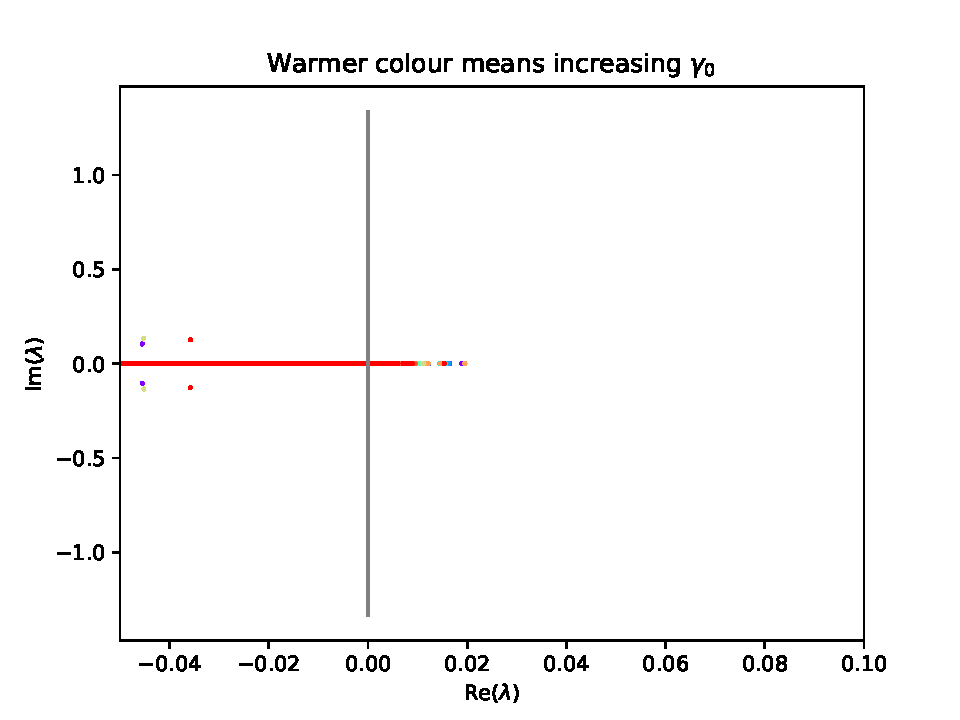
\includegraphics[width=\textwidth]{eigenspectrum_heterogeneous_eff_closeup.png}
			\subcaption{With a heterogeneous $\sigma$.}
		\end{subfigure}
		\caption{Close up of the eigenspectrum distribution of the jacobian at a feasible equilibrium where the $\gamma_{ij}$ have been picked normally (mean $\gamma_0$, small variance) for the same number of simulations. We see that with a homogeneous $\sigma$, dynamical stability is ensured as no positive eigenvalues are observed, as was shown in \cite{Butler:2018aa}. Introducing heterogeneity in $\sigma$ however seems to always lead to some instability as positive eigenvalues are found.}\label{fig : effect heterogeneity stability}
	\end{figure}
	\begin{figure}
		\centering
		\begin{subfigure}{0.49\textwidth}
			\includegraphics[width=\textwidth]{eigenspectrum_homogenous_eff.png}
			\subcaption{With a homogenous $\sigma$.}
		\end{subfigure}
		\begin{subfigure}{0.49\textwidth}
			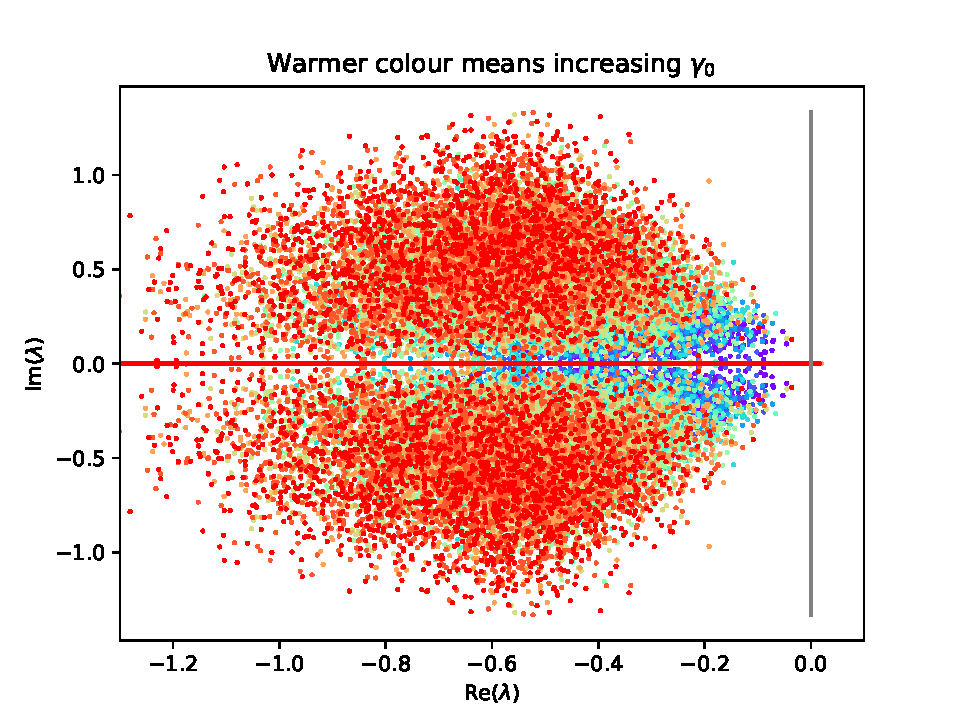
\includegraphics[width=\textwidth]{eigenspectrum_heterogeneous_eff.png}
			\subcaption{With a heterogeneous $\sigma$.}
		\end{subfigure}
		\caption{Full eigenspectrum distribution of the jacobian at a feasible equilibrium where the $\gamma_{ij}$ have been picked normally (mean $\gamma_0$, small variance) for the same number of simulations. Adding heterogeneity seems to lower the multiplicity of the eigenvalues (as we observe more distinct points for the same total number of non distinct eigenvalues). Note also that increasing $\gamma_0$, i.e. make the species eat more, seems to lower the mean eigenvalue. }\label{fig : effect heterogeneity eigenspectrum}
	\end{figure}

	\clearpage
	\section{The one-resource case}
	We take the special case $N_R = 1$ and $N_S$ arbitrary. Looking at the equilibrium equations \eqref{eq : equilibrium condition 1} and \eqref{eq : equilibrium condition 2} yields directly two solutions:
	\begin{itemize}
		\item $S^*_i = 0 $ for every species and $R^* = \frac{\lambda}{\mu}$. That is the case where eventually every species dies out (we will call it trivial equilibrium).
		\item $S^*_i = 0$ for every species but one (denote it $k$) and then $$R^* = \frac{\delta_k}{\sigma_k \gamma_k}  \text{ and } S^*_k = \frac{\mu R^* - \lambda}{\alpha_k - \gamma_k R^*}$$
	\end{itemize}

	In the one resource case, the jacobian is given by
	\begin{equation}
		J =
		\begin{pmatrix}
			- \mu - \gamma \cdot S & -\gamma^T R + \alpha \\
			\sigma_i \gamma_i S_i & \delta_{ij}(\sigma_i \gamma_i R - \delta_i)
		\end{pmatrix}
	\end{equation}
		\subsection{The trivial equilibrium}
	In that case, every species dies out in the end, such that $S^*_i = 0$ $\forall i = 1,\dots, N_S$. The jacobian at equilibrium is then given by:
	\begin{equation}
		J^* =
		\begin{pmatrix}
			- \mu & -\gamma^T R^* + \alpha \\
			0 & \delta_{ij}(\sigma_i \gamma_i R^*-\delta_i)
		\end{pmatrix}
	\end{equation}
		\subsection{The non trivial equilibrium}
	In the non trivial equilibrium, one of the species survives, which gives the following jacobian at equilibrium:
	\begin{equation}
		J^* =
		\begin{pmatrix}
			-\mu-\gamma_k S^*_k & -\gamma^T R^*+\alpha \\
			\delta_{ik} \sigma_i \gamma_i S^*_i & \delta_{ij}(\sigma_i \gamma_i R^*-\delta_i)
		\end{pmatrix}.
	\end{equation}

	For instance if $N_S=2$ and that $k=2$ (ie the survivor is the last species), the Jacobian matrix would be :
	\begin{equation}
		J^* =
		\begin{pmatrix}
			-\mu-\gamma_2 S^*_2 & -\gamma_1 R^* + \alpha_1 & -\gamma_2 R^* +\alpha_2 \\
			0 & \sigma_1 \gamma_1 R^*-\delta_1 & 0 \\
			\sigma_2 \gamma_2 S^*_2 & 0 & \sigma_2 \gamma_2 R^* - \delta_2
		\end{pmatrix}
		=
		\begin{pmatrix}
			-\mu-\gamma_2 S^*_2 & -\gamma_1 R^* + \alpha_1 & -\gamma_2 R^* +\alpha_2 \\
			0 & \sigma_1 \gamma_1 R^*-\delta_1 & 0 \\
			\sigma_2 \gamma_2 S^*_2 & 0 & 0
		\end{pmatrix}
	\end{equation}
	Note that this result is more general than the one in the paper by Butler since we accept solutions where some species simply disappear (contrarily to their assumptions when deriving the equilibria). This here changes the game since it makes the lower block of the jacobian matrix not zero anymore.

	Without loss of generality we can put the non vanishing species at the end and hence the jacobian at equilibrium generally looks like :
	\begin{equation}
		J^* =
		\begin{pmatrix}
			-a & \vect{b}^T \\
			\vect{c} & D
		\end{pmatrix}
	\end{equation}
	where:
	\begin{itemize}
		\item $a = \mu+\gamma_{N_S} S^*_{N_S}$ is a positive number.
		\item $\vect{b}$ is a $N_S$ vector defined by $b_i = - \gamma_i R^* + \alpha_i$.
		\item $\vect{c}$ is a vector who is mostly zero. More explicitly, $c_i = \delta_{iN_S} \sigma_i \gamma_i S^*_i$.
		\item $D$ is a $N_S \times N_S$ diagonal matrix. Explicitly,
		$$D = \text{diag}(\sigma_1 \gamma_1 R^*-\delta_1, \dots,\sigma_{N_S-1} \gamma_{N_S-1} R^*-\delta_{N_S-1}, 0)$$
	\end{itemize}
		\subsection{Stability of the non trivial equilibrium}
	We now seek the solution to the equation $\det(J^*-\lambda)=0$ (there is a bit of confusion here, since until the eigenspectrum is fully written down, $\lambda$ refers to the eigenvalues and not the $\lambda$ of the model). Explicitly, it is:
	\begin{equation}
		\det
		\begin{pmatrix}
			-a-\lambda & \vect{b}^T \\
			\vect{c} & D-\lambda
		\end{pmatrix}
		=0 \label{eq : block matrix equilibrium one resource}
	\end{equation}
	Assuming that $\lambda \neq -a$, this can be rewritten as:
	\begin{equation}
		\left(-\lambda-a\right)\det\left(D-\lambda-\vect{c}\left(-\lambda-a\right)^{-1}\vect{b}^T\right) = 0 \iff \det\left(D-\lambda-\vect{c}\left(-\lambda-a\right)^{-1}\vect{b}^T\right) =0
	\end{equation}
	Assuming a finite $\lambda$ this is equivalent to:
	\begin{equation}
		\det\left(\left(-\lambda-a\right)\left(D-\lambda\right)-\vect{c}\vect{b}^T\right) = \det\left(\lambda^2+(a-D)\lambda-(aD+\vect{c}\vect{b}^T)\right)=0.
		\label{eq: defines lambda}
	\end{equation}
	Using the famous equality $\det M=\exp\Tr\ln M$, Eq.\eqref{eq: defines lambda}
	can be written as
	\begin{equation}
		\Tr\left(\ln\left(\lambda^2+(a-D)\lambda-(aD+\vect{c}\vect{b}^T)\right)\right)=-\infty.
	\end{equation}
	Explicitly:
	\begin{align}
		& \sum_{i=1}^{N_S} \ln\left(\lambda^2+(a-D_i) \lambda - (aD+\vect{c}\vect{b}^T)_i\right) = -\infty \\
		\implies& \ln\left(\prod_{i=1}^{N_S} \lambda^2+(a-D_i) \lambda - (aD+\vect{c}\vect{b}^T)_i\right) = -\infty \\
		\implies& \prod_{i=1}^{N_S} \left(\lambda^2+(a-D_i) \lambda - (aD+\vect{c}\vect{b}^T)_i\right) =0 \\
		\implies& \left(\lambda^2+a\lambda-c_{N_S}b_{N_S}\right)\prod_{i=1}^{N_S-1} \left(\lambda^2+(a-D_i) \lambda - aD_i\right)  =0 \\
		\implies& \left(\lambda-\frac{a}{2}\left(\sqrt{1+\frac{4 c_{N_S} b_{N_S}}{a^2}}-1\right)\right)\left(\lambda+\frac{a}{2}\left(\sqrt{1+\frac{4 c_{N_S} b_{N_S}}{a^2}}+1\right)\right)
			\prod_{i=1}^{N_S-1}\left(\lambda-D_i\right) =0
	\end{align}
	So the spectrum of the Jacobian is given by the $N_S+1$ values:
	\begin{equation}
		\sigma(J^*) = \left\{\sigma_i \gamma_i R^*-\delta_i, i=1,..., N_S-1\right\} \cup \left\{\frac{a}{2}\left(\sqrt{1+\frac{4c_{N_S} b_{N_S}}{a^2}}-1\right), -\frac{a}{2}\left(\sqrt{1+\frac{4c_{N_S} b_{N_S}}{a^2}}+1\right)\right\}
	\end{equation}
	With the full spectrum in hand, we can now define a stability condition : we say the equilibrium is stable is stable when every eigenvalue has a negative real part.
	This implies first of all :
	\begin{equation}
		\frac{4 c_{N_S} b_{N_S}}{a^2} < 0 \iff c_{N_S} b_{N_S} < 0 \iff b_{N_S} < 0 \iff R^* = \frac{\delta_{N_S}}{\sigma_{N_S}\gamma_{N_S}} > \frac{\alpha_{N_s}}{\gamma_{N_S}}
	\end{equation}
	It also implies
	\begin{equation}
		\sigma_i \gamma_i R^* - \delta_i < 0 \ \ \forall i = 1, \dots, N_S-1 \iff R^* = \frac{\delta_{N_S}}{\sigma_{N_S}\gamma_{N_S}} < \min_{i \in \{1, \dots, N_S-1\}}\left(\frac{\delta_i}{\sigma_i \gamma_{i}} \right)
	\end{equation}
	Hence we must have
	\begin{equation}
		\boxed{ \frac{\alpha_{N_s}}{\gamma_{N_S}} < R^* < \min_{i \in \{1, \dots, N_S-1\}}\left(\frac{\delta_i}{\sigma_i \gamma_{i}}\right)}
	\end{equation}
	for the equilibrium to be stable.


	Let's now assume $\lambda = -a$ and see if Eq.\eqref{eq : block matrix equilibrium one resource} still holds. If we assume $\lambda=-a$, then Eq.\eqref{eq : block matrix equilibrium one resource} becomes :
	\begin{equation}
	\det
	\begin{pmatrix}
		0 & \vect{b}^T\\
		\vect{c} & D+a
	\end{pmatrix} =0
	\end{equation}
	Keeping in mind that the only non-zero entry in $\vect{c}$ is the last one, thanks to the Laplace expansion of the determinant, this equation becomes:
	\begin{equation}
		\det
		\begin{pmatrix}
			\vect{b}^T \\
			\tilde{D}
		\end{pmatrix}
		=
		\det
		\begin{pmatrix}
			b_1 & \dots & b_{N_S} \\
			\tilde{D}_1 & 0 & 0 \\
			0 & \ddots & 0 \\
			0 & 0 & \tilde{D}_{N_S-1}
		\end{pmatrix}
		=0, \label{eq : reduced determinant}
	\end{equation}
	where $\tilde{D}$ is a $(N_S-1)\times(N_S-1)$ diagonal matrix whose entries are given by $\tilde{D}_i = \sigma_i \gamma_i R^* - \delta_i +a$. Eq.\eqref{eq : reduced determinant} can be further simplified using again Laplace expansion:
	\begin{equation}
		b_1 \det
		\begin{pmatrix}
			0 & \dots & \dots& 0 \\
			\tilde{D}_2 & \ddots & & \\
			 & \ddots & \ddots & \\
			&  & \tilde{D}_{N_S-1} & 0
		\end{pmatrix}
		- \tilde{D_1} \det
		\begin{pmatrix}
			b_2 & \dots & b_{N_S} \\
			\tilde{D}_2 &  0 & 0 \\
			0 & \ddots & 0 \\
			0 & 0 & \tilde{D}_{N_S-1}
		\end{pmatrix} = 0
	\end{equation}
	Since the first term of this is clearly zero, we see that :
	\begin{equation}
		\det
		\begin{pmatrix}
			b_1 & \dots & b_{N_S} \\
			\tilde{D}_1 & 0 & 0 \\
			0 & \ddots & 0 \\
			0 & 0 & \tilde{D}_{N_S-1}
		\end{pmatrix} = 0 \iff \tilde{D_1} \det
		\begin{pmatrix}
			b_2 & \dots & b_{N_S} \\
			\tilde{D}_2 &  0 & 0 \\
			0 & \ddots & 0 \\
			0 & 0 & \tilde{D}_{N_S-1}
		\end{pmatrix} = 0
	\end{equation}
	By a recursive reasoning we conclude that
	\begin{equation}
		\det
		\begin{pmatrix}
			\vect{b}^T \\
			\tilde{D}
		\end{pmatrix}
		= 0 \iff \prod_{i=1}^{N_S-1} \tilde{D}_i =0
	\end{equation}
	And hence $-a$ is part of the eigenspectrum if and only if one of the $D_i$ $(i=1, \dots, N_S-1)$ is equal to $-a$.

	Note that although the way to get this result is not super rigorous mathematically (the formula $\det M = \exp\left(\Tr\left(\ln M\right)\right)$ has been used in places it really should not), the results still hold (you can obtain the same values for the eigenvalues by using properties of the determinant and of the matrix).

	\clearpage
	\section{Solvable cases}
		\paragraph{Specialist consumers} We consider the case of a system with $N_S = N_R$ and each species eats one resource, that it does not share with anyone. Without loss of generality we can say that species $S_i$ feeds from resource $R_\alpha$. We also take $\alpha_{\alpha i}$ lower triangular, which biologically means that species $S_i$ releases biomass in resources $R_\alpha$ with $\alpha > i$ (i.e. $S_1$ releases to $R_1, \dots, R_{N_R}$, $S_2$ to $R_2, \dots, R_{N_R}$ and so on). Mathematically, these conditions translate to
		\begin{equation}
			\alpha_{\alpha j} = 0 \text{ if } \alpha < j \text{ and } \gamma_{i\alpha} = \delta_{i\alpha} \gamma_{i\alpha}
		\end{equation}
		With such definitions, we see clearly that $\beta$ is diagonal while $\Gamma$ is lower triangular, which means that if we choose $Z$ to be lower triangular, $A(\lambda)$ is also lower triangular, meaning that Eq.\eqref{eq : lambda equation} is easily solvable :
		\begin{equation}
		\det\left(A(\lambda)-\lambda\right) = 0 \iff \prod_i^{N_S} \left(A_{ii}(\lambda)-\lambda\right)=0 \iff \prod_i^{N_S}\left(Z_{ii}+\frac{\beta_{ii}\Gamma_{ii}}{D_i + \lambda}-\lambda\right)=0.
		\end{equation}
		This gives $N_S$ equations characterizing $\lambda$ :
		\begin{align}
			& Z_{ii}+\frac{\beta_{ii}\Gamma_{ii}}{D_i + \lambda}-\lambda = 0 \\
			\iff & \lambda^2 + \left(D_i-Z_{ii}\right) \lambda-\left(\beta_{ii}\Gamma_{ii}+Z_{ii}D_i\right) = 0 \\
			\iff & \lambda = \frac{Z_{ii}-D_i \pm \sqrt{\left(D_i+Z_{ii}\right)^2 + 4 \beta_{ii} \Gamma_{ii}}}{2}.
		\end{align}
		This means the full spectrum of $N_S + N_R = 2 N_S$ eigenvalues is given by :
		\begin{equation}
			\sigma(J^*) = \left\{\frac{Z_{ii}-D_i + \sqrt{\left(D_i+Z_{ii}\right)^2 + 4 \beta_{ii} \Gamma_{ii}}}{2}, \frac{Z_{ii}-D_i - \sqrt{\left(D_i+Z_{ii}\right)^2 + 4 \beta_{ii} \Gamma_{ii}}}{2} \text{ with } i = 1, \dots, N_S\right\}
		\end{equation}
		A stability condition on the equilibrium is then directly found :
		\begin{equation}
			\max_{i = 1, \dots, N_S}\Re\left(Z_{ii}-D_i + \sqrt{\left(D_i+Z_{ii}\right)^2 + 4 \beta_{ii} \Gamma_{ii}}\right) < 0. \label{eq : stability condition}
		\end{equation}
		We assume that the index $k$ is the one giving the maximum value of $\Re\left(Z_{ii}-D_i + \sqrt{\left(D_i+Z_{ii}\right)^2 + 4 \beta_{ii} \Gamma_{ii}}\right)$.
		We also assume $Z_{kk}=0$. Then we know the system is unstable if :
		\begin{equation}
			-D_{k}+\Re\left(\sqrt{D_k^2+ 4 \beta_{kk} \Gamma_{kk}}\right) > 0
		\end{equation}
		This is achieved if and only if:
		\begin{equation}
			\Gamma_{kk} > 0
		\end{equation}
		Hence we clearly see that the stability condition Eq.\eqref{eq : stability condition} is:
		\begin{equation}
			\text{ The system is dynamically stable } \iff \Gamma \text{ has non positive entries.}
		\end{equation}
		Comparison between Fig.\ref{fig : max max eigenvalue} and Fig.\ref{fig : mean max eigenvalue} tends to show that when $\Gamma$ is fully negative, the system is fully stable, as expected. The slight deviation in the mean is because of the number of random variables picked : even if the upper boundary of the interval is positive, the matrix may contain only negative elements. That zone should disappear as $N_R$ increases and we pick more random variables (i.e. more chances of picking a positive one), which is indeed what we observe in Fig.\ref{fig : mean max eigenvalue}
		\begin{figure}
			\centering
			\begin{subfigure}{0.49\textwidth}
				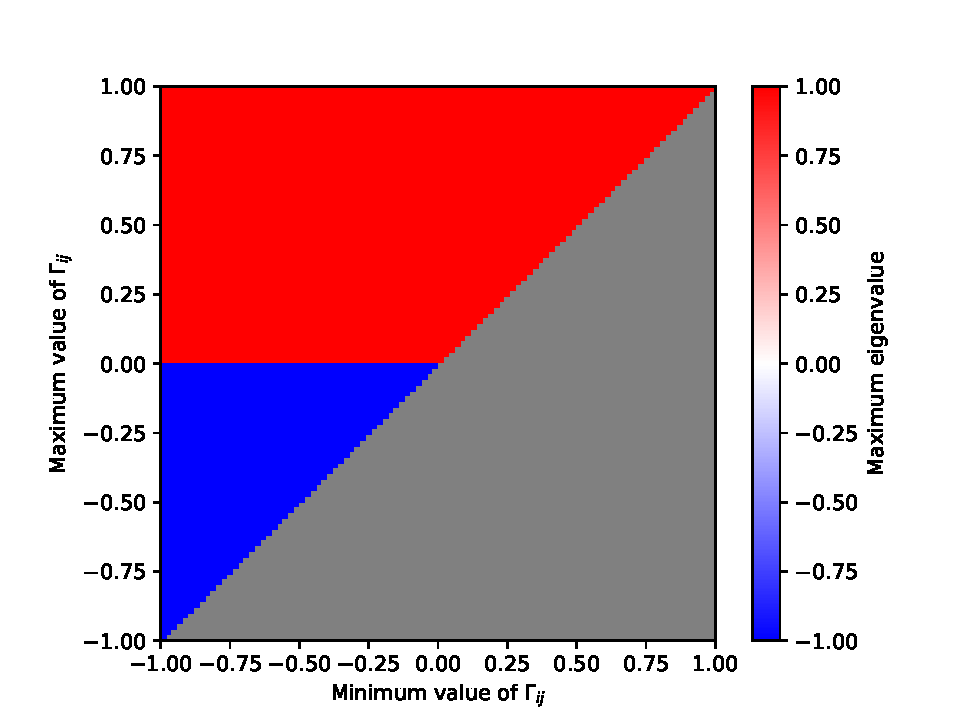
\includegraphics[width=\linewidth]{max_maximum_eigval_wrto_Gamma_NR=3.pdf}
				\subcaption{$N_R = 3$}
			\end{subfigure}
			\hfill
			\begin{subfigure}{0.49\textwidth}
				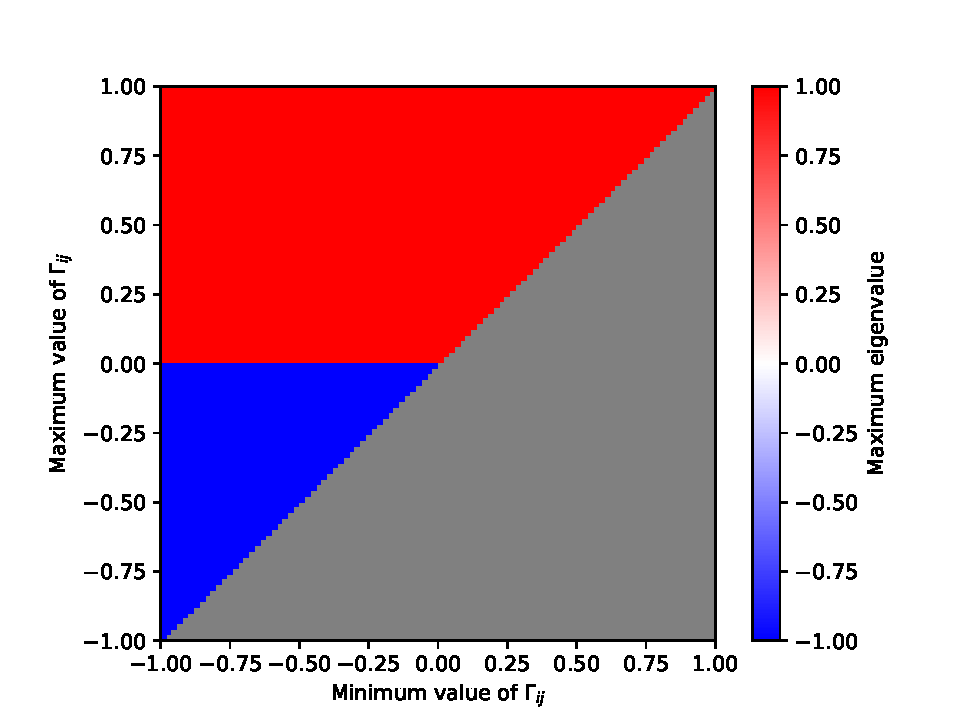
\includegraphics[width=\linewidth]{max_maximum_eigval_wrto_Gamma_NR=8.pdf}
				\subcaption{$N_R = 8$}
			\end{subfigure}
			\caption{Sign of the maximal maximum eigenvalue picked over 300 simulations for each point, according to parameters describing the distribution of the entries of the triangular $\Gamma$ matrix. More specifically each non-zero entry is picked uniformly over the given interval. We clearly observe a transition from stable to unstable systems.} \label{fig : max max eigenvalue}
		\end{figure}
		\begin{figure}
			\centering
			\begin{subfigure}{0.49\textwidth}
				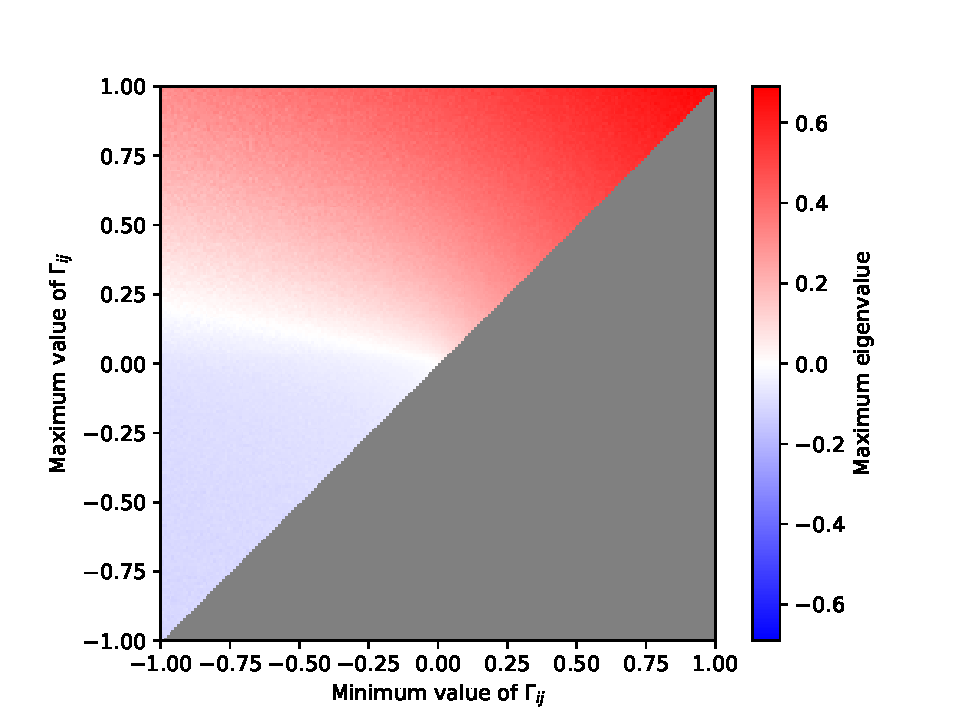
\includegraphics[width=\linewidth]{mean_maximum_eigval_wrto_Gamma_NR=3.pdf}
				\subcaption{$N_R = 3$}
			\end{subfigure}
			\hfill
			\begin{subfigure}{0.49\textwidth}
				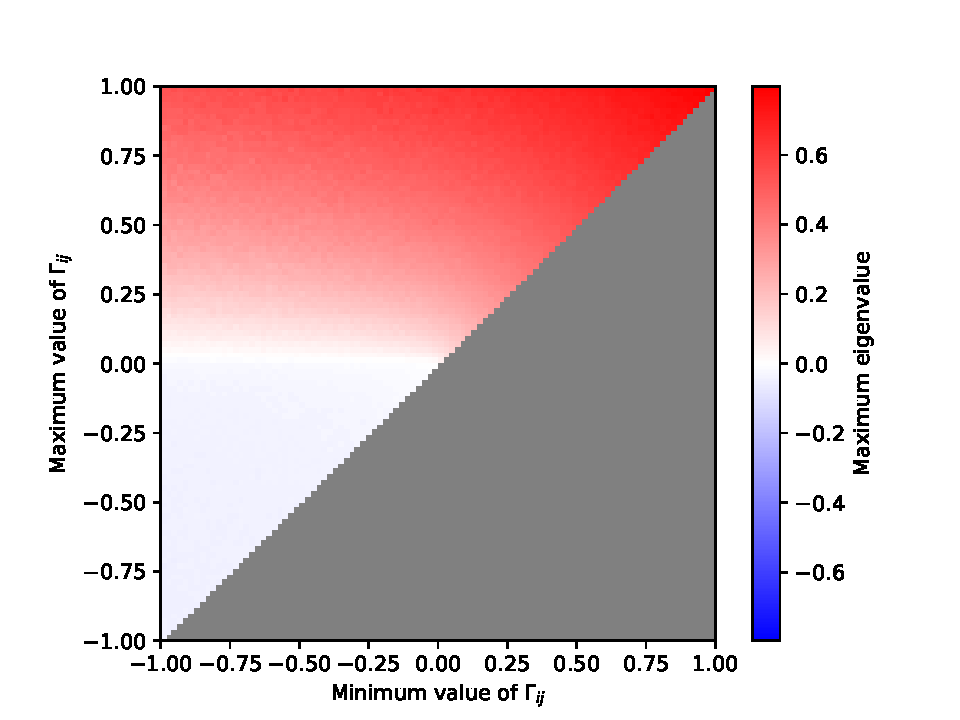
\includegraphics[width=\linewidth]{mean_maximum_eigval_wrto_Gamma_NR=8.pdf}
				\subcaption{$N_R = 8$}
			\end{subfigure}
			\caption{Average maximum eigenvalue (over 300 simulations for each point) according to parameters describing the distribution of the entries of the triangular $\Gamma$ matrix. More specifically each non-zero entry is picked uniformly over the given interval. We clearly observe a transition from stable to unstable systems.} \label{fig : mean max eigenvalue}
		\end{figure}
\end{document}
